\documentclass{article}

\usepackage{fancyhdr}
\usepackage{braket}
\usepackage{extramarks}
\usepackage{amsmath}
\usepackage{amsthm}
\usepackage{amsfonts}
\usepackage{tikz}
\usepackage[plain]{algorithm}
\usepackage{algpseudocode}
\usepackage{mathtools}
\usepackage{graphicx}
\graphicspath{ {./Images/} }

\DeclarePairedDelimiter\abs{\lvert}{\rvert}%
\DeclarePairedDelimiter\norm{\lVert}{\rVert}%

\makeatletter
\let\oldabs\abs
\def\abs{\@ifstar{\oldabs}{\oldabs*}}
%
\let\oldnorm\norm
\def\norm{\@ifstar{\oldnorm}{\oldnorm*}}
\makeatother

\newcommand*{\Value}{\frac{1}{2}x^2}%

\usetikzlibrary{automata,positioning}

%
% Basic Document Settings
%

\topmargin=-0.45in
\evensidemargin=0in
\oddsidemargin=0in
\textwidth=6.5in
\textheight=9.0in
\headsep=0.25in

\linespread{1.1}

\pagestyle{fancy}
\lhead{\hmwkAuthorName}
\chead{\hmwkClass\ (\hmwkClassInstructor\ \hmwkClassTime): \hmwkTitle}
\rhead{\firstxmark}
\lfoot{\lastxmark}
\cfoot{\thepage}

\renewcommand\headrulewidth{0.4pt}
\renewcommand\footrulewidth{0.4pt}

\setlength\parindent{0pt}

%
% Create Problem Sections
%

\newcommand{\enterProblemHeader}[1]{
    \nobreak\extramarks{}{Problem \arabic{#1} continued on next page\ldots}\nobreak{}
    \nobreak\extramarks{Problem \arabic{#1} (continued)}{Problem \arabic{#1} continued on next page\ldots}\nobreak{}
}

\newcommand{\exitProblemHeader}[1]{
    \nobreak\extramarks{Problem \arabic{#1} (continued)}{Problem \arabic{#1} continued on next page\ldots}\nobreak{}
    \stepcounter{#1}
    \nobreak\extramarks{Problem \arabic{#1}}{}\nobreak{}
}

\setcounter{secnumdepth}{0}
\newcounter{partCounter}
\newcounter{homeworkProblemCounter}
\setcounter{homeworkProblemCounter}{1}
\nobreak\extramarks{Problem \arabic{homeworkProblemCounter}}{}\nobreak{}

%
% Homework Problem Environment
%
% This environment takes an optional argument. When given, it will adjust the
% problem counter. This is useful for when the problems given for your
% assignment aren't sequential. See the last 3 problems of this template for an
% example.
%
\newenvironment{homeworkProblem}[1][-1]{
    \ifnum#1>0
        \setcounter{homeworkProblemCounter}{#1}
    \fi
    \section{Problem \arabic{homeworkProblemCounter}}
    \setcounter{partCounter}{1}
    \enterProblemHeader{homeworkProblemCounter}
}{
    \exitProblemHeader{homeworkProblemCounter}
}

%
% Homework Details
%   - Title
%   - Due date
%   - Class
%   - Section/Time
%   - Instructor
%   - Author
%

\newcommand{\hmwkTitle}{Homework\ \#10}
\newcommand{\hmwkDueDate}{April 7, 2020}
\newcommand{\hmwkClass}{Physics 926}
\newcommand{\hmwkClassTime}{}
\newcommand{\hmwkClassInstructor}{Professor Ken Bloom}
\newcommand{\hmwkAuthorName}{\textbf{Robert Tabb}}

%
% Title Page
%

\title{
    \vspace{2in}
    \textmd{\textbf{\hmwkClass:\ \hmwkTitle}}\\
    \normalsize\vspace{0.1in}\small{Due\ on\ \hmwkDueDate\ at 5pm}\\
    \vspace{0.1in}\large{\textit{\hmwkClassInstructor\ \hmwkClassTime}}
    \vspace{3in}
}

\author{\hmwkAuthorName}
\date{}

\renewcommand{\part}[1]{\textbf{\large Part \Alph{partCounter}}\stepcounter{partCounter}\\}

%
% Various Helper Commands
%

% Useful for algorithms
\newcommand{\alg}[1]{\textsc{\bfseries \footnotesize #1}}

% For derivatives
\newcommand{\deriv}[1]{\frac{\mathrm{d}}{\mathrm{d}x} (#1)}

% For partial derivatives
\newcommand{\pderiv}[2]{\frac{\partial}{\partial #1} (#2)}

% Integral dx
\newcommand{\dx}{\mathrm{d}x}

% Alias for the Solution section header
\newcommand{\solution}{\textbf{\large Solution}}

% Probability commands: Expectation, Variance, Covariance, Bias
\newcommand{\E}{\mathrm{E}}
\newcommand{\Var}{\mathrm{Var}}
\newcommand{\Cov}{\mathrm{Cov}}
\newcommand{\Bias}{\mathrm{Bias}}

\begin{document}

\maketitle

\pagebreak

\begin{homeworkProblem}
	Show that:
	\[
		\frac{\Gamma(K_L \rightarrow \pi^-e^+\nu_e)-\Gamma(K_L \rightarrow \pi^+e^-\bar{\nu}_e))}{\Gamma(K_L \rightarrow \pi^-e^+\nu_e)+\Gamma(K_L \rightarrow \pi^+e^-\bar{\nu}_e))} = 2Re(\epsilon)
	\]
	to first order in $\epsilon$. This asymmetry is evidence for indirect CP violation, and also allows us to unambiguously define electric charge - positive charge is assigned to the lepton that dominates in the $K_L$ decay.
	\\
	\\
	\textbf{Solution}
	\\
	\\
	\[
		\ket{K_L}=\frac{1}{\sqrt{1+\abs{\epsilon}}}\left[\frac{1+\epsilon}{\sqrt{2}}\ket{K^0}-\frac{1-\epsilon}{\sqrt{2}}\ket{\bar{K}^0}\right] 
	\]
	
	$\bar{K^0} \rightarrow \pi^+e^-\bar{\nu}_e$ and $K^0 \rightarrow \pi^-e^+\nu_e$ (see Figure \ref{kaons}), therefore to get $K_L \rightarrow \pi^+e^-\bar{\nu}_e$, take the inner product of $\bar{K^0}$ with $K_L$ and to get $K_L \rightarrow \pi^-e^+\nu_e$, take the inner product of $K^0$ with $K_L$.
	
	\begin{figure}[h]
		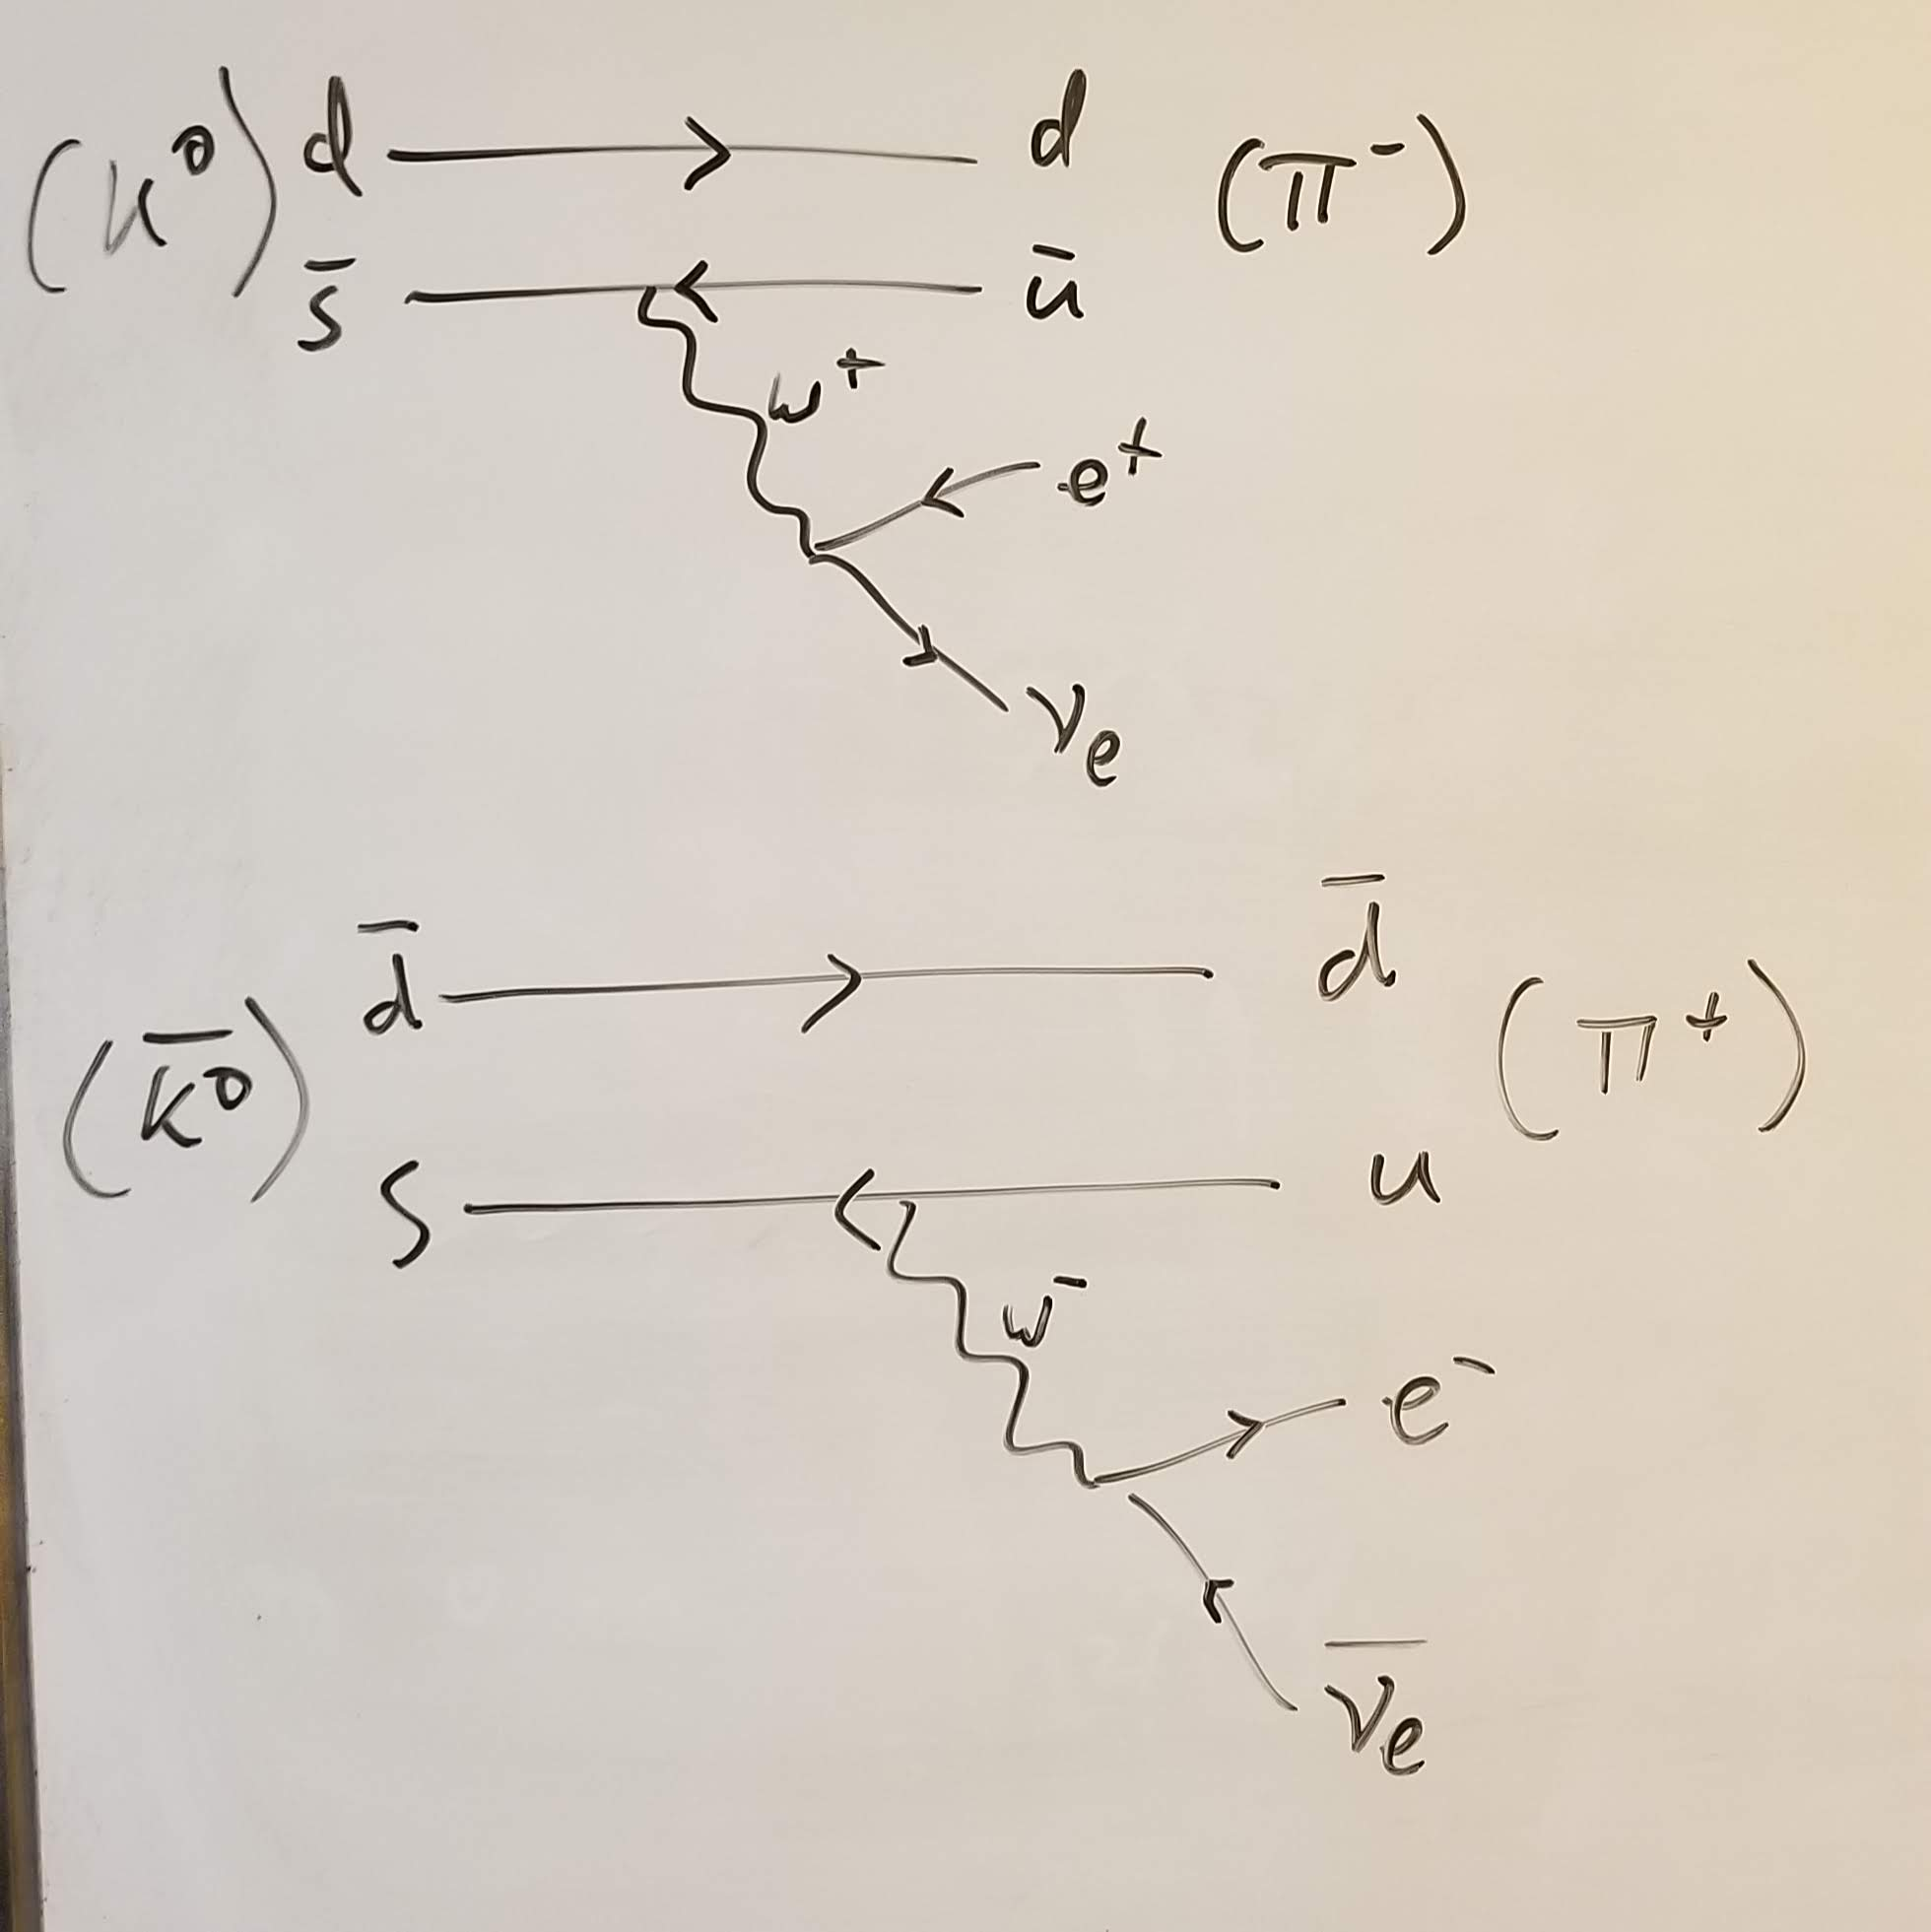
\includegraphics[scale=0.2]{kaons}
		\centering
		\caption{The two neutral kaon decays}
		\label{kaons}
		\centering
	\end{figure}
	
	\[
		\begin{split}
		\Gamma(K_L \rightarrow \pi^+e^-\bar{\nu}_e) \propto \abs{\braket{\bar{K}^0|K_L}}^2 \propto \abs{1-\epsilon}^2=(1-\epsilon)(1-\epsilon^*)=1-\epsilon^*-\epsilon+\abs{\epsilon}^2 \approx 1-2Re(\epsilon) \\ 
		\Gamma(K_L \rightarrow \pi^-e^+\nu_e) \propto \abs{\braket{K^0|K_L}}^2 \propto \abs{1+\epsilon}^2=(1+\epsilon)(1+\epsilon^*)=1+\epsilon^*+\epsilon+\abs{\epsilon}^2 \approx 1+2Re(\epsilon)
		\end{split}
	\]
	Here I dropped the $\epsilon^2$ term since we are only looking to first order in $\epsilon$. I also dropped any constants since they will be the same for each term and will divide out in the end.
	\[
		\begin{split}
		\frac{\Gamma(K_L \rightarrow \pi^-e^+\nu_e)-\Gamma(K_L \rightarrow \pi^+e^-\bar{\nu}_e))}{\Gamma(K_L \rightarrow \pi^-e^+\nu_e)+\Gamma(K_L \rightarrow \pi^+e^-\bar{\nu}_e))} =& \frac{1+2Re(\epsilon)-(1-2Re(\epsilon))}{1+2Re(\epsilon)+(1-2Re(\epsilon))}\\
		=&\frac{4Re(\epsilon)}{2} = 2Re(\epsilon)
		\end{split}
	\]
	
\end{homeworkProblem}

\pagebreak

\begin{homeworkProblem}
	Defining
	\[
		\eta_{\pm}=\abs{\eta_\pm}e^{i\phi_\pm}=\frac{\braket{\pi^+\pi^-|K_L}}{\braket{\pi^+\pi^-|K_S}}
	\]
	calculate the probabilities of $\pi^+\pi^-$ decay as a function of proper time for an initial $K^0$ or $\bar{K^0}$ produced at $t=0$. Express your answer, up to common proportionality constants, in terms of $\epsilon,\abs{\eta_\pm},\phi_\pm,\Delta m, \Gamma_S,$ and $\Gamma_L$, where $\Delta m = K_S - K_L$. Keep only leading terms in $\epsilon$. Using the experimental values for these quantities, plot the two probabilities as a function of time in units of the $K_S$ lifetime, going out to 30 $K_S$ lifetimes.	
	\\
	\\
	\textbf{Solution}
	\\
	\\
	Here are the definitions of $K_L$ and $K_S$ in terms of $K^0$ and $\bar{K^0}$:
	\[
		\begin{split}
		\ket{K_L}=\frac{1}{\sqrt{1+\abs{\epsilon}}}\left[\frac{1+\epsilon}{\sqrt{2}}\ket{K^0}-\frac{1-\epsilon}{\sqrt{2}}\ket{\bar{K^0}}\right] \\
		\ket{K_S}=\frac{1}{\sqrt{1+\abs{\epsilon}}}\left[\frac{1+\epsilon}{\sqrt{2}}\ket{K^0}+\frac{1-\epsilon}{\sqrt{2}}\ket{\bar{K^0}}\right] 
		\end{split}	
	\]

	And here they are in terms of the CP eigenstates:
	\[
		\begin{split}
		\ket{K_L}=\frac{1}{\sqrt{1+\abs{\epsilon}}}\left[\ket{K_2}+\epsilon \ket{K_1}\right] \\
		\ket{K_S}=\frac{1}{\sqrt{1+\abs{\epsilon}}}\left[\ket{K_1}+\epsilon \ket{K_2}\right] 
		\end{split}
	\]
	First, define the time-evolution of the wave function in the same way it was done in the lecture notes: 
	\[
		\begin{split}
		\ket{K_S(t)}=&\ket{K_S}e^{im_St-\Gamma_St/2} \\
		\ket{K_L(t)}=&\ket{K_L}e^{im_Lt-\Gamma_Lt/2} \\
		\end{split}
	\]
	We know that the$\pi^+\pi^-$ is a CP eigenstate with eigenvalue of +1. So to project $K_L$ or $K_S$ onto $\pi^+\pi^-$ we project onto $K_1$:
	\[
		\begin{split}
		\braket{\pi^+\pi^-|K_L} = \braket{K_1|K_L}=\frac{\epsilon}{\sqrt{1+\abs{\epsilon}}}e^{im_Lt-\Gamma_Lt/2} \\
		\braket{\pi^+\pi^-|K_L} = \braket{K_1|K_S}=\frac{1}{\sqrt{1+\abs{\epsilon}}}e^{im_St-\Gamma_St/2}
		\end{split}
	\]
	So now we have:
	\[
		\begin{split}
		\frac{\braket{\pi^+\pi^-|K_L}}{\braket{\pi^+\pi^-|K_S}} =& \epsilon e^{i(m_L-m_s)t+\frac{1}{2}(\Gamma_S-\Gamma_L)t} \\
		=& \epsilon e^{-i\Delta mt+\frac{1}{2}(\Gamma_S-\Gamma_L)t} \\
		=& \abs{\eta_\pm}e^{i\phi_\pm}
		\end{split}
	\]
	The subscript on the wave function state refers to the initial beam being either purely $K^0$ or purely $\bar{K^0}$.
	Here I will rewrite the wave functions in terms of the CP eigenstates because the $\pi^+\pi^-$ system is a CP eigenstate with eigenvalue of +1 and we can use this:
	\[
		\begin{split}
				\ket{\psi(t)}_{K^0}=& \frac{1}{\sqrt{2}}\left[\ket{K_S(t)} + \ket{K_L(t)} \right] \\
				=& \frac{1}{\sqrt{2}}\left[\ket{K_S}e^{im_St-\Gamma_St/2} + \ket{K_L}e^{im_Lt-\Gamma_Lt/2}\right] \\
				\ket{\psi(t)}_{\bar{K^0}}=& \frac{1}{\sqrt{2}}\left[\ket{K_S}e^{im_St-\Gamma_St/2} - \ket{K_L}e^{im_Lt-\Gamma_Lt/2}\right] \\
		\ket{\psi(t)}_{K^0}=&\frac{1}{\sqrt{2}}\frac{1}{\sqrt{1+\abs{\epsilon}}}\left[  (\ket{K_1}+\epsilon \ket{K_2})e^{im_St-\Gamma_St/2} + (\ket{K_2}+\epsilon\ket{K_1})e^{im_Lt-\Gamma_Lt/2}\right] \\
		=& \frac{1}{\sqrt{2}}\frac{1}{\sqrt{1+\abs{\epsilon}}}\left[ (e^{im_St-\Gamma_St/2}+\epsilon e^{im_Lt-\Gamma_Lt/2})\ket{K_1}+(e^{im_Lt-\Gamma_Lt/2}+\epsilon e^{im_St-\Gamma_St/2})\ket{K_2}\right] \\
		\ket{\psi(t)}_{\bar{K^0}}=& \frac{1}{\sqrt{2}}\frac{1}{\sqrt{1+\abs{\epsilon}}}\left[ (e^{im_St-\Gamma_St/2}-\epsilon e^{im_Lt-\Gamma_Lt/2})\ket{K_1}+(-e^{im_Lt-\Gamma_Lt/2}+\epsilon e^{im_St-\Gamma_St/2})\ket{K_2}\right]
		\end{split}
	\] 
	
\end{homeworkProblem}

\pagebreak

\begin{homeworkProblem}

\end{homeworkProblem}

\pagebreak

\begin{homeworkProblem}

\end{homeworkProblem}

\end{document}
